\section{Independent Factorization for Graph-based Representation Parsing}
\label{sec:lex-phr:factorization-analysis}

In this chapter, we mainly study the parsing on four meaning
representations~(DM, PSD, AMR, and UCCA) and an application-specific
representation TOP on dialogue parsing. According to the brief
introduction for them in~\label{ssec:bg:broad-mr}, we have mentioned
the anchoring type for each representation. In this section, we will
first revisit the anchoring analysis for them, epsecially we show the
detailed evidences that AMR is actually implicit
lexical-anchoring. Then, we group the five representations into two
groups: Lexical Anchoring~(DM, PSD, AMR) and Phrasal Anchoring~(UCCA
and TOP), and finally we consider the structural inductive biases into
the independent factorization for each group.

\subsection{Anchoring Analysis}
\label{ssec:lex-phr:anchoring-analysis}
The 2019 Conference on Computational Language Learning~(CoNLL) hosted
a shared task on Cross-Framework Meaning Representation
Parsing~\cite[MRP 2019,][]{Oep:Abe:Haj:19}, which encourage
participants in building a parser for five different meaning
representations in three distinct flavors. \texttt{Flavor-0} includes
the DELPH-IN MRS Bi-lexical Dependencies~\cite[DM,][]{ivanova2012did}
and Prague Semantic
Dependencies~\cite[PSD,][]{hajic2012announcing,miyao2014house}. Both
frameworks under this representation have a syntactic backbone that is
(either natively or by-proxy) based on bi-lexical dependency
structures. As a result, the semantic concepts in these meaning
representations can be anchored to the individual lexical units of the
sentence. Hence, \texttt{Flavor-0} is actually explicit
\textbf{Lexical-Anchoring}. Hence, \texttt{Flavor-0} is actually
Lexical-Anchoring in our thesis.

\texttt{Flavor-1} includes Elementary Dependency
Structures~\cite[EDS,][]{oepen2006discriminant} and Universal
Conceptual Cognitive Annotation
framework~\cite[UCCA,][]{abend2013universal}, which shows an explicit,
many-to-many anchoring of semantic concepts onto sub-strings of the
underlying sentence. In this thesis, we only consider UCCA with
another application-specific symbolic representation TOP, where the
underlying sub-strings mainly forms a tree-like structures. We grouped
UCCA and TOP as \textbf{Phrasal-Anchoring}.

Finally, \texttt{Flavor-2} includes Abstract Meaning
Representation~\cite[AMR,][]{Banarescu:LWPjKI7N}, which is designed to
abstract the meaning representation away from its surface token. But
it leaves open the question of how these are derived. In the following
part, we mainly analyze the detailed anchoring analysis of AMR.

\subsubsection{Anchoring Analysis for AMR}
\label{sssec:lex-phr:amr-anchor}
Previous studies have shown that the nodes in AMR graphs are
predominantly aligned with the surface lexical units, although
explicit anchoring is absent from the AMR representation.  In this
section, we review the related work supporting the claim of the
implicit anchoring in AMR is actually lexical-anchoring, which can be
merged into \texttt{Flavor-0} when we consider the parsing methods on
it.

\Paragraph{AMR-to-String Alignments} A straightforward solution to
find the missing anchoring in an AMR Graph is to align it with a
sentence; We denote it as AMR-to-String alignment. ISI
alignments~\cite{Pourdamghani:2014aligning} first linearizes the AMR
graph into a sequence, and then use IBM word alignment
model~\cite{brown1993mathematics} to align the linearized sequence of
concepts and relations with tokens in the sentence. According to the
AMR annotation guidelines and error analysis of ISI aligner, some of
the nodes or relations are evoked by subwords, e.g., the whole graph
fragment \texttt{(p/possible-01 :polarity -)} is evoked by word
``impossible", where the subword \texttt{\char`\"im-\char`\"} actually
evoked the relation polarity and concept \texttt{\char`\"-\char`\"};
On the other side, sometimes concepts are evoked by multiple words,
e.g., named entities, \texttt{(c/city :name (n/name :op1
  \char`\"New\char`" :op2 \char`\"York\char`\"))}, which also happens
in explict anchoring of DM and PSD. Hence, aligning and parsing with
recategorized graph fragments are a natural solution in aligners and
parsers. JAMR aligner~\cite{Flanigan:2014vc} uses a set of rules to
greedily align single tokens, special entities and a set of multiple
word expression to AMR graph fragments, which is widely used in
previous AMR
parsers~\cite[\eg][]{Flanigan:2014vc,Wang:2015uo,Artzi:2009tb,Pust:2015ug,Peng:2015tj,Konstas:2017uj,Wang:2017vt}. Other
AMR-to-String Alignments exists, such as the extended HMM-based
aligner. To consider more structure info in the linearized AMR
concepts, \citet{Wang:2017vt} proposed a Hidden Markov
Model~(HMM)-based alignment method with a novel graph distance. All of
them report over 90\% F-score on their own hand-aligned datasets,
which shows that AMR-to-String alignments are almost token-level
anchoring.

\Paragraph{AMR-to-Dependency Alignments} \citet{chen2017unsupervised}
first tries to align an AMR graph with a syntactic dependency tree.
\citet{szubert2018structured} conducted further analysis on dependency
tree and AMR interface. It showed 97\% of AMR edges can be evoked by
words or the syntactic dependency edges between words.  Those nodes in
the dependency graph are anchored to each lexical token in the
original sentence. Hence, this observation indirectly shows that AMR
nodes can be aligned to the lexical tokens in the sentence.

Both AMR-to-String and AMR-to-dependency alignments shows that AMR
nodes, including recategorized AMR graph fragements, do have implicit
lexical anchoring. Based on this, \citet{lyu2018amr} propose to treat
token-node alignments as discrete and exclusive alignment matrix and
learn the latent alignment jointly with parsing. Recently,
attention-based seq2graph model also achieved the state-of-the-art
accuracy on AMR parsing~\cite{zhang-etal-2018-stog}.  However, whether
the attention weights can be explained as AMR alignments needs more
investigation in future.

%

\subsubsection{Summary of Anchoring Analysis}

\Paragraph{Explicit Lexical Anchoring: DM and PSD}
As discussed in~\autoref{ssec:bg:bi-leixcal}, DM and PSD aims to
represent all the semantic dependencies between words with fully
covering the senentence. For each node in the graph, there will be an
explicit words, multiword expression align to it. Hence, we call such
kind of lexical anchoring as explicit lexical-anchoring.

\Paragraph{Implicit Lexical Anchoring: AMR}
AMR tries to abstract the meaning representation away from the surface
token. The absense of explicit anchoring can present difficulties for
parsing. However, through extensive anchoring analysis on AMR
alignments, we show that AMR nodes can be implicitly aligned to the
leixical tokens or special entities in a sentence. Hence, we mainly
consider the lexical-level input decomposition for AMR.

\Paragraph{Phrasal Anchoring: UCCA and TOP} According to the
background of UCCA~\S\ref{ssec:bg:ucca}, UCCA non-teriminal node are
aligned to phrases in a sentence. Hence, we need to consider
pharse-level input decomposition for UCCA.

\subsection{Independent Factorization on Lexical-Anchoring}
\label{ssec:lex-phr:lex-factorization-analysis}

According the linguistic analysis on anchoring, we have show that DM,
PSD and AMR belongs to the lexical-anchoring, which indicates that
their nodes in the output graph are explicitly or implicitly anchored
to the lexical units of the corresponding input sentence.  Before
showing the unified design of independent factorization, let us
introduce the fundamental concepts and notations. We refer to words in
a sentence as $x=(x_{0};x_{1};...x_{i};...;x_{n})$, where $n$ is the
sentence length.  For all the graph-based representations in our
lexical-anchoring category, we decompose the whole graph into nodes
and edges. We denotes the labelled nodes~(concepts) as
$C = \{c_{i}\mid i \in [0,m]\}$, where $m$ is the number of concepts.
While the labelled edges~(relations) between the $m$ concepts are
denoted as $R = \{r_{ij}\mid i \in [0, m], j \in [0, m]\}$.  $r_{ij}$ means
the directional relation from the node $i$ to the node $j$.  We use
$r_{ij}=\Phi$ to indicate no edge from the node $i$ to the node $j$.

In this part, based on the above notations, we introduce how to
independent factorization on lexical-anchoring by addressing the three
main chellenges in \textbf{Output
  Decomposition}~(\S\ref{sssec:lex-phr:lex-output-decomposition}),
\textbf{Input Decomposition and Alignments
  Discovery}~(\S\ref{sssec:lex-phr:lex-input-decomposition}), and
\textbf{Factor
  Modelling}~(\S\ref{sec:lex-phr:graph-based},\S\ref{sec:lex-phr:cky-based})
%\begin{figure}[t]
%\centering
%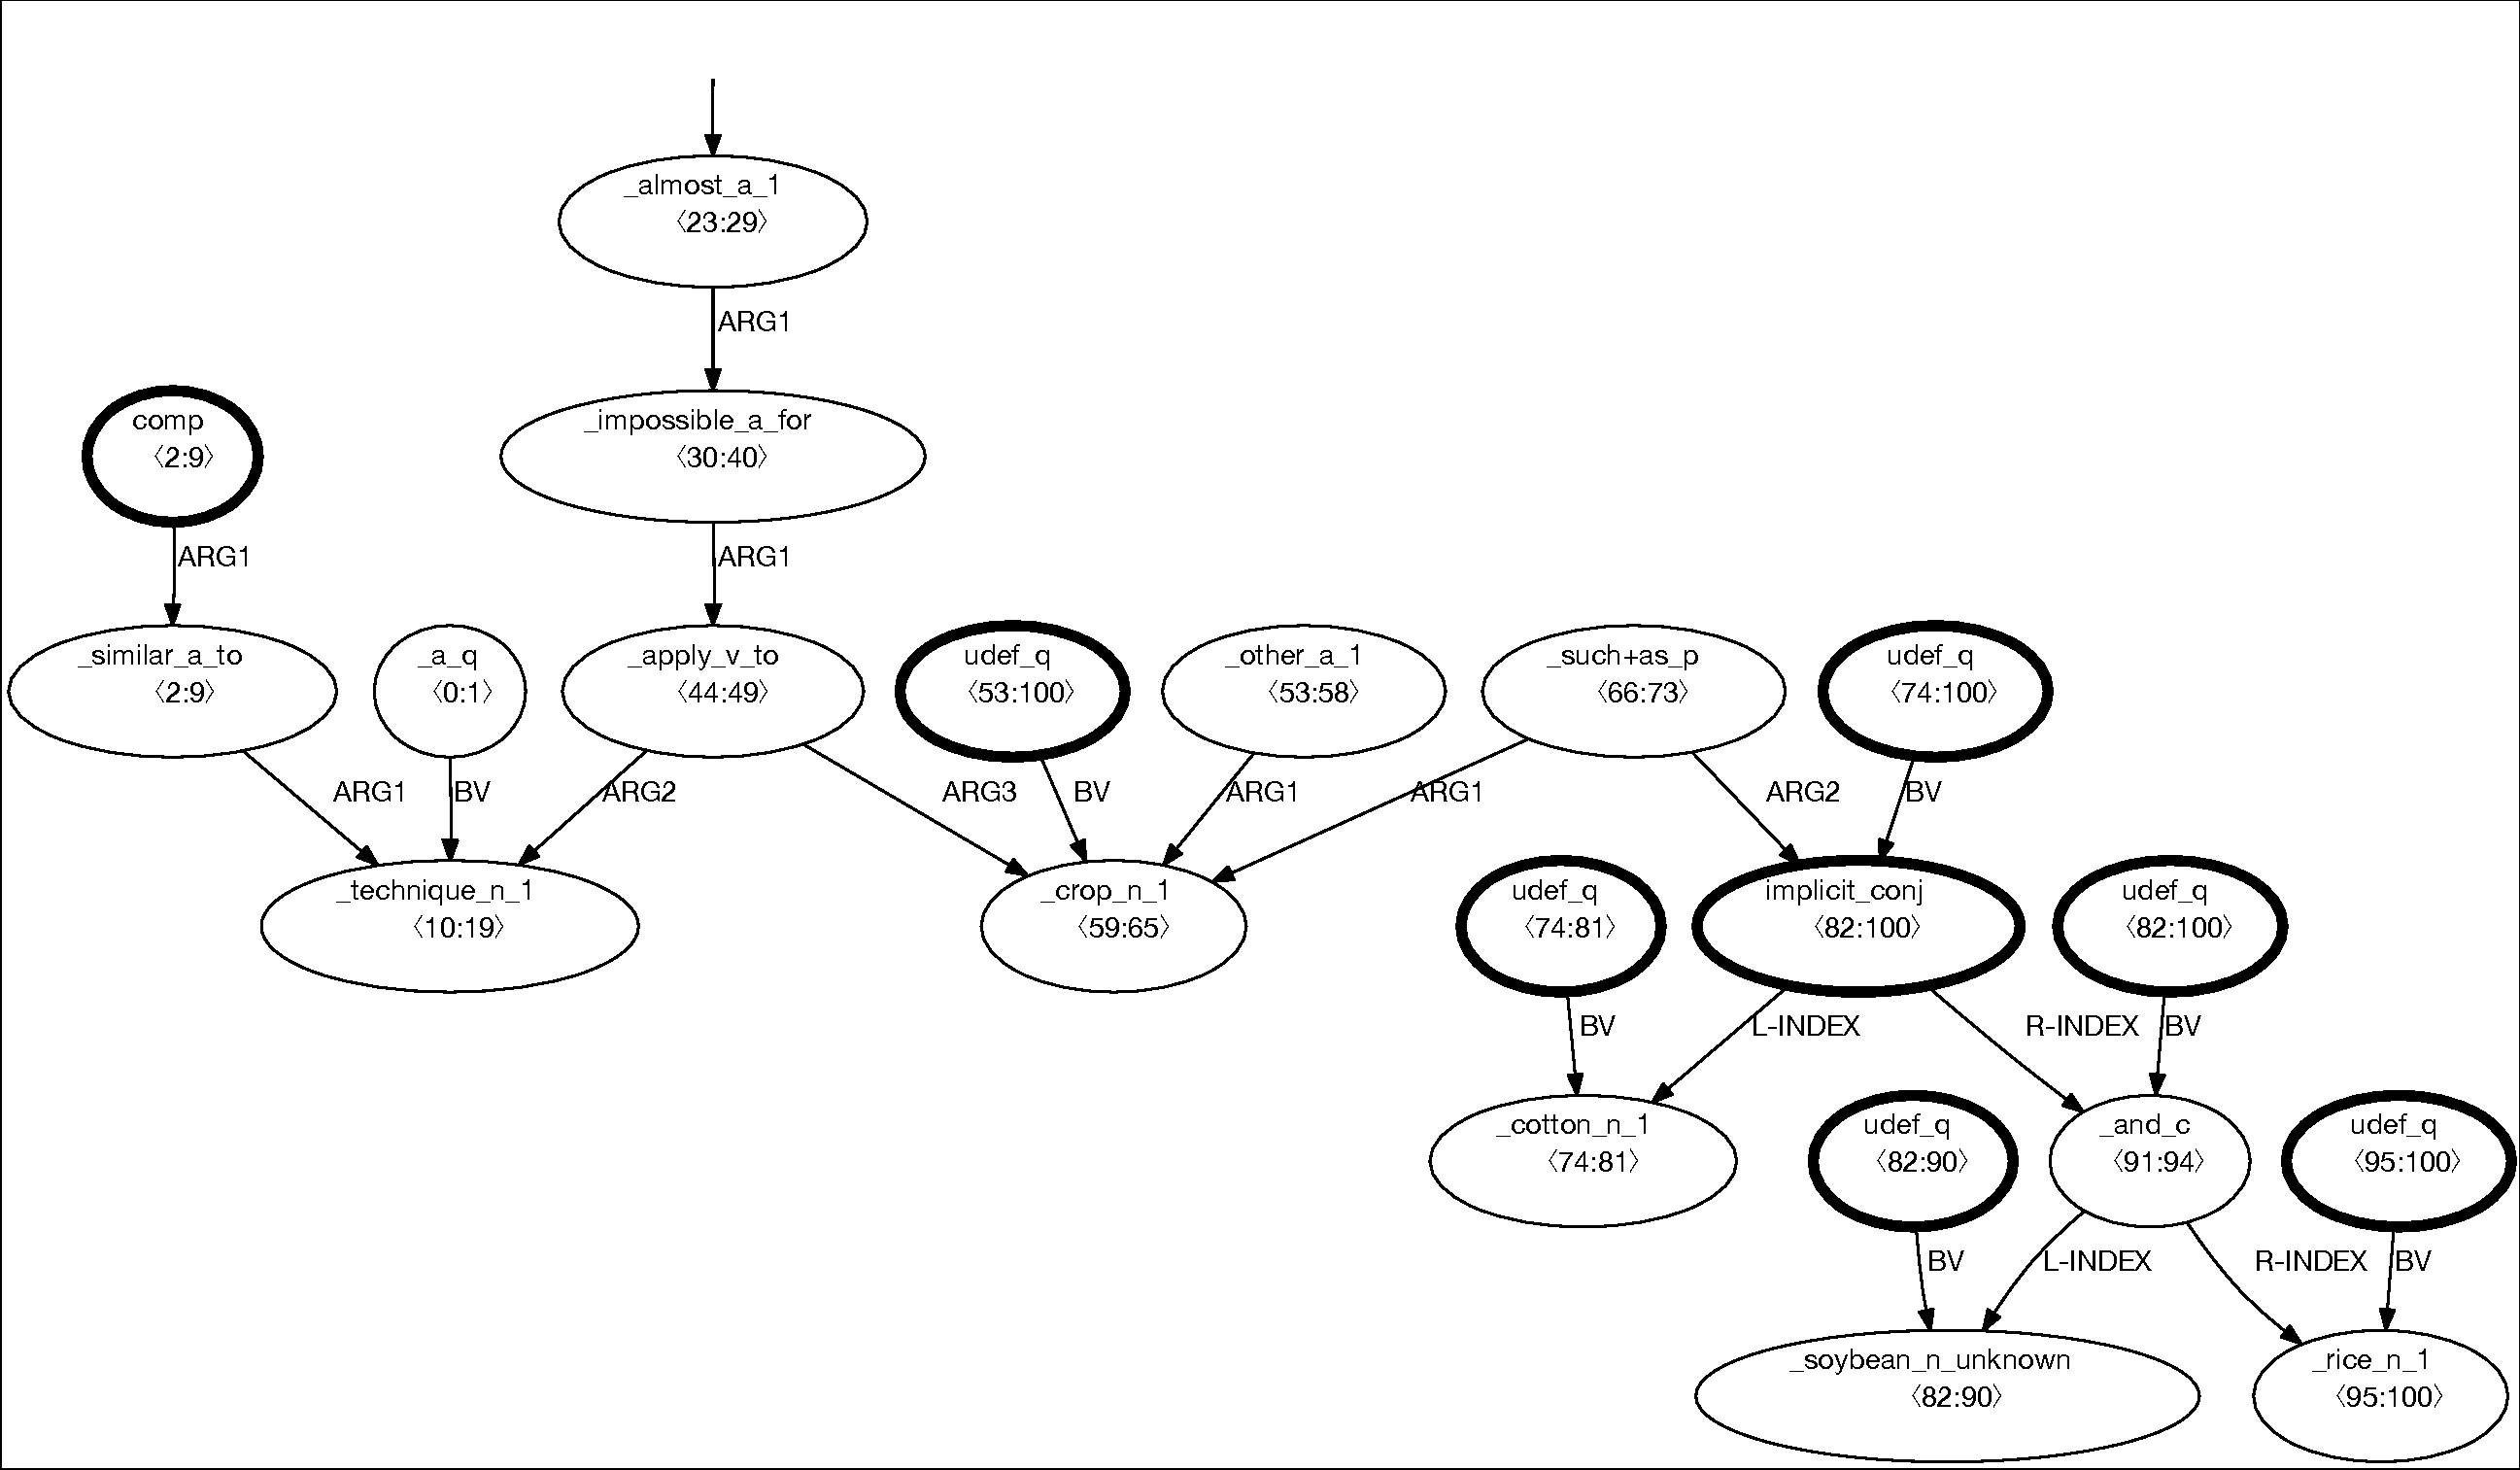
\includegraphics[width=.96\textwidth,trim=.1cm .1cm .05cm .05cm, clip]{eds-white.pdf}
%\caption{\label{fig:phrasal-anchoring}Phrasal-anchoring in
%  EDS[wsj\#0209013], for the sentence \texttt{\char`\"A similar
%    technique is almost impossible to apply to other crops, such as
%    cotton, soybeans and rice.\char`\"}. Bold nodes are similar to the
%  non-terminal nodes in UCCA, which are anchored multiple tokens, thus
%  overlapping with the anchors of other nodes.}
%\end{figure}
\subsubsection{Output Decomposition}
\label{sssec:lex-phr:lex-output-decomposition}
For the lexical-anchoring grah-based representations~(DM, PSD, AMR),
the target graph can be decomposed into independent nodes or
subgraphs. For DM and PSD, each node in the target graph is strictly
aligned to the correspnding tokon. Hence, we simple decompose the DM
and PSD graph by nodes. However, when we introduce the necessary of
strutural inductive biases for independent factorization~\S
\ref{sssec:intro:structural-biases}, the AMR parsing running examples
shows that we need specially handle those special h



\subsubsection{Input Decomposition and Alignments Discovery}
\label{sssec:lex-phr:lex-input-decomposition}
According to the bi-lexical dependency structures of DM and PSD, and
implicit lexical token anchoring on AMR, the nodes/categorized graph
fragments of DM, PSD, and AMR are anchored to surface lexical units in
an explicit or implict way. Especially, those lexical units do not
overlap with each other, and most of them are just single tokens,
multiple word expression, or named entities. In other words, when
parsing a sentence into DM, PSD, AMR graphs, tokens in the original
sentence can be merged by looking up a lexicon dict when preprocessing
and then may be considered as a single token for aligning or parsing.

\subsubsection{Factor Modelling}
\label{sssec:lex-phr:factor-modelling}




\subsection{Independent Factorization on Phrasal-Anchoring}
\label{ssec:lex-phr:phr-factorization-analysis}

As a result, the semantic concepts in these meaning
representations can be anchored to the individual lexical units of the
sentence. \texttt{Flavor-1} includes Elementary Dependency
Structures~\cite[EDS,][]{oepen2006discriminant} and Universal
Conceptual Cognitive Annotation
framework~\cite[UCCA,][]{abend2013universal}, which shows an explicit,
many-to-many anchoring of semantic concepts onto sub-strings of the
underlying sentence.

However, different from the lexical anchoring without overlapping,
nodes in EDS and UCCA may align to larger overlapped word spans which
involves syntactic or semantic pharsal structure. Nodes in UCCA do not
have node labels or node properties, but all the nodes are anchored to
the spans of the underlying sentence. Furthermore, the nodes in UCCA
are linked into a hierarchical structure, with edges going between
parent and child nodes. With certain exceptions~(e.g. remote edges),
the majority of the UCCA graphs are tree-like structures. According to
the position as well as the anchoring style, nodes in UCCA can be
classified into the following two types:

\begin{inparaenum}
\item \textbf{Terminal nodes} are the leaf semantic
  concepts anchored to individual lexical units in the sentence

\item \textbf{Non-terminal nodes} are usually anchored to a span with
  more than one lexical units, thus usually overlapped with the
  anchoring of terminal nodes.
\end{inparaenum}

The similar classification of anchoring nodes also applies to the
nodes in EDS, although they do not regularly form a recursive tree
like UCCA. As the running example in Figure
\ref{fig:phrasal-anchoring}, most of the nodes belongs to terminal
nodes, which can be explicitly anchored to a single token in the
original sentence. However, those bold non-teriminal nodes are
anchored to a large span of words. For example, the node
\texttt{\char`\"undef\_q\char`\"} with span \texttt{<53:100>} is
aligned to the whole substring starting from ``other crops" to the
end; The abstract node with label \texttt{imp\_conj} are corresponding
to the whole coordinate structure between \texttt{soybeans and rice}

\subsection{Summary of Factorization Analysis}
\label{ssec:lex-phr:summary-anchoring}

In summary, by treating AMR as an implicitly lexically anchored MR, we
propose a simplified taxonomy for parsing the five meaning
representations.

\Paragraph{\texttt{Lexical-anchoring}: DM, PSD, AMR}
In~\autoref{sec:lex-phr:graph-based}, we proposed an unified
graph-based parsing framework for \texttt{lexical-anchoring}, which
use a latent alignment model to support both the explicit and implicit
alignments.

\Paragraph{\texttt{Phrasal-anchoring}: UCCA, TOP}
In~\autoref{sec:lex-phr:cky-based}, we proposed an unified span-based
CKY parsing for both UCCA and TOP.

%%% Local Variables:
%%% mode: latex
%%% TeX-master: "../../thesis-main.ltx"
%%% End:
